\documentclass[12pt,letter]{article}


\usepackage{nicefrac,amsmath}
\usepackage[english]{babel}
\usepackage{helvet}
\usepackage{enumerate}
\usepackage{parskip}
%\usepackage{apacite}
\usepackage[english]{babel}
\usepackage{booktabs}
\usepackage[top=1in, bottom=1in, left=1in, right=1in]{geometry}
\usepackage{graphicx}
\usepackage{subfigure}
\usepackage{url}
\usepackage{hyperref}
\usepackage{physics}
\usepackage{cancel}
\usepackage{gensymb}
\usepackage{bbm}
\usepackage{dsfont}
\usepackage{mathtools}
\usepackage{appendix}
\usepackage{etoolbox}

% Inserts \clearpage before \begin{appendices}
\BeforeBeginEnvironment{appendices}{\clearpage}

\usepackage{algpseudocode}
\usepackage{algorithm}


\usepackage[usenames,dvipsnames]{color}
 \usepackage{listings}
 \definecolor{Brown}{cmyk}{0,0.81,1,0.60}
 \definecolor{OliveGreen}{cmyk}{0.64,0,0.95,0.40}
 \definecolor{CadetBlue}{cmyk}{0.62,0.57,0.23,0}



 \lstset{language=C,%basicstyle=\normalsize,
 keywordstyle=\ttfamily\color{OliveGreen}\bfseries,
 identifierstyle=\ttfamily\color{CadetBlue}\bfseries, 
 commentstyle=\color{Brown}\ttfamily,
 stringstyle=\ttfamily\color{red},
 showstringspaces=false}


\newcommand{\argmax}[1]{\underset{#1}{\operatorname{arg}\,\operatorname{max}}\;}
\newcommand{\argmin}[1]{\underset{#1}{\operatorname{arg}\,\operatorname{min}}\;}

% Coordinate frame curly bracket notation 
\newcommand{\Frame}[1]{Frame $\left\{{#1}\right\}$}

\usepackage{cmbright}
\usepackage[T1]{fontenc}

\setlength{\parskip}{12pt} % 1ex plus 0.5ex minus 0.2ex}

%\renewcommand{\familydefault}{\sfdefault}

\setlength{\parindent}{0cm}
\renewcommand{\baselinestretch}{1.2}

\title{{\bf Forward Kinematics}}

\date{}
\begin{document}
\maketitle
\vspace{-1.0in}

%{\small 
%\tableofcontents
%\listoffigures
%\listofalgorithms
%}

%\newpage



\begin{figure}[ht]
	\begin{center}
			{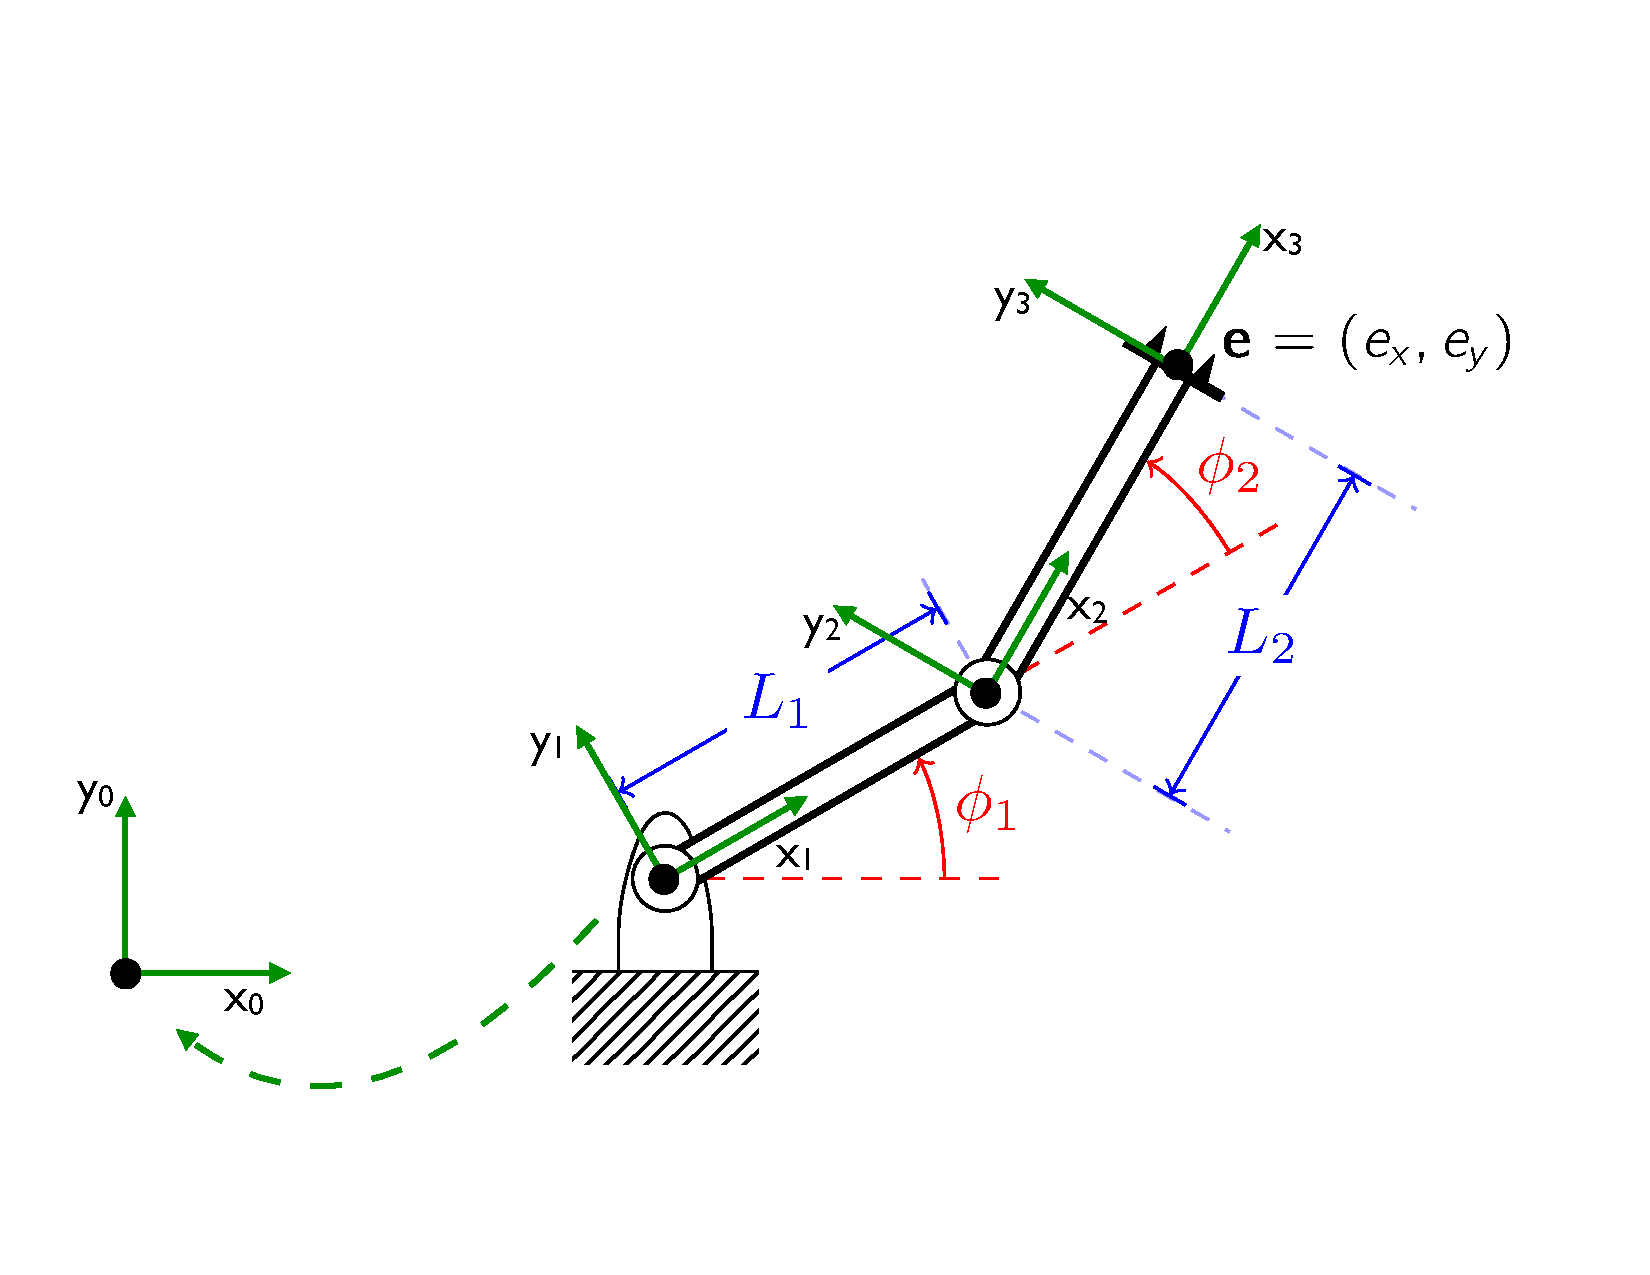
\includegraphics[width=.80\textwidth]{figs/robotArm01}}
	\end{center}
	\caption{A two-dimensional articulated arm. }
	\label{frames01}
\end{figure}

Consider the arm structure shown in Figure \ref{frames01}. Assume the following values for the arm configuration: the location of the first joint (i.e., the one attached to the ground support) is ${\bf p}_1 = \left(3,2\right)^\mathsf{T}$, the lengths of the parts are $L_1 = 5$ and  $L_2 = 8$.
\begin{enumerate}
	\item  Write the matrices that represent the local coordinate frames $\{1\}$, $\{2\}$, and $\{3\}$. These frames are indicated in green in Figure \ref{frames01}. The transformations you need to write are $T_{0,1}$, $T_{1,2}$, and $T_{2,3}$.
	\item Write the matrices that represent each local frame w.r.t. the global frame $\{0\}$. The transformations you need to write are $T_{0,1}$, $T_{0,2}$, and $T_{0,3}$.
	\item Use the transformation matrices to obtain the global coordinates (i.e., w.r.t. frame $\{0\}$) of the following points under the given joint-angle configurations: 
	\begin{itemize}
		\item The middle point of each part, for $\phi_1 = pi/8$ and $\phi_2 = pi/4$. Draw the configuration of the arm under these parameters. 
		\item All the joint points and the end effector, for $\phi_1 = pi/4$ and $\phi_2 = pi/8$. Draw the configuration of the arm under these parameters. 
		\item Write the matrix that represents the coordinate frame of the end effector w.r.t. frame  $\{1\}$, i.e., $T_{1,3}$
		\item Write the matrix that represents the coordinate frame $\{1\}$ w.r.t. to the frame of the end effector.
	\end{itemize}
\end{enumerate}



\end{document}
% end of file template.tex




